\documentclass[14pt]{article}
\usepackage[utf8]{inputenc}
\usepackage[T2A]{fontenc}
\usepackage[russian]{babel} % Кириллица uchun, lekin matn lotin yozuvida
\usepackage{amsmath, amssymb}
\usepackage{geometry}
\usepackage{graphicx}
\usepackage{xcolor}
\usepackage{hyperref}
\usepackage{tasks}
\usepackage{tcolorbox}
\tcbuselibrary{skins, breakable, theorems}
\usepackage{fancyhdr}
\usepackage{lastpage}
\usepackage{enumitem}
\usepackage{paracol}
\usepackage{ifthen}
\usepackage{needspace}

% Определение команд для тангенса и котангенса (русский стиль)
\newcommand{\tg}{\operatorname{tg}}
\newcommand{\ctg}{\operatorname{ctg}}

% Настройка геометрии
\geometry{a4paper, left=10mm, right=10mm, top=20mm, bottom=20mm, headheight=15pt}

% Цветовая палитра
\definecolor{primary}{RGB}{52, 152, 219}
\definecolor{secondary}{RGB}{46, 204, 113}
\definecolor{accent}{RGB}{155, 89, 182}
\definecolor{lightbg}{RGB}{248, 249, 250}
\definecolor{taskborder}{RGB}{230, 230, 230}
\definecolor{optionbg}{RGB}{240, 242, 245}

% Основной фон страницы
\pagecolor{lightbg}

% Настройка гиперссылок
\hypersetup{
    colorlinks=true,
    linkcolor=primary,
    urlcolor=primary,
}

% Колонтитулы
\pagestyle{fancy}
\fancyhf{}
\fancyhead[L]{\textcolor{primary}{\textbf{MathCore | MOCK Test-10}}}
\fancyhead[R]{\textcolor{secondary}{Abdunazarov M.X.}}
\fancyfoot[L]{\href{https://t.me/Math_Core_Dtm_MS_Att}{\textcolor{primary}{MathCore}}}
\fancyfoot[R]{\href{https://t.me/Abd_mardon}{\textcolor{secondary}{@Abd\_mardon}}}
\fancyfoot[C]{\textcolor{gray}{\thepage/\pageref{LastPage}}}
\renewcommand{\headrulewidth}{0.5pt}
\renewcommand{\headrule}{\hbox to\headwidth{\color{primary}\leaders\hrule height \headrulewidth\hfill}}
\renewcommand{\footrulewidth}{0.5pt}
\renewcommand{\footrule}{\hbox to\headwidth{\color{secondary}\leaders\hrule height \footrulewidth\hfill}}

% Титульная страница
\title{\Huge \textbf{\textcolor{primary}{MOCK Test-10}}}
\author{\textcolor{secondary}{Abdunazarov M.X.}}
\date{}
\newenvironment{dd}{\begin{center}}{\end{center}}
% Стиль для карточки вопроса
\newtcolorbox{questionbox}[2][]{
    enhanced,
    breakable,
    colback=white,
    colframe=primary,
    coltitle=white,
    fonttitle=\bfseries\large,
    title={Задача \hfill \textcolor{white}{#2}},
    attach boxed title to top left={xshift=5mm, yshift=-2mm},
    boxed title style={size=small, colback=primary, sharp corners},
    sharp corners,
    boxrule=0.5pt,
    left=5mm,
    right=5mm,
    top=5mm,
    bottom=5mm,
    drop fuzzy shadow,
    #1
}

% Стиль для вариантов ответов
\newlist{options}{enumerate}{1}
\setlist[options]{
    label=\textbf{\Alph*)},
    leftmargin=*,
    itemsep=2pt,
    topsep=5pt,
    before={\vspace{2mm}\begin{tcolorbox}[
        colback=optionbg,
        colframe=white,
        sharp corners,
        boxrule=0pt,
        left=2mm,
        right=2mm,
        top=2mm,
        bottom=2mm,
    ]},
    after={\end{tcolorbox}\vspace{2mm}},
}

% Для рисунков
\newcommand{\questionimage}[2][0.5\linewidth]{%
    \begin{center}
        \includegraphics[width=#1]{#2}
    \end{center}
}

% Для удобства: команда вставки вопроса с рисунком
\newcommand{\questionitem}[4]{%
    \needspace{5cm}
    \begin{questionbox}{#1}
        #2
        \ifx&#3&%
        \else
            \questionimage{#3}
        \fi
        \begin{options}
            #4
        \end{options}
    \end{questionbox}
}

\begin{document}

% Титульная страница
\maketitle
\begin{center}
    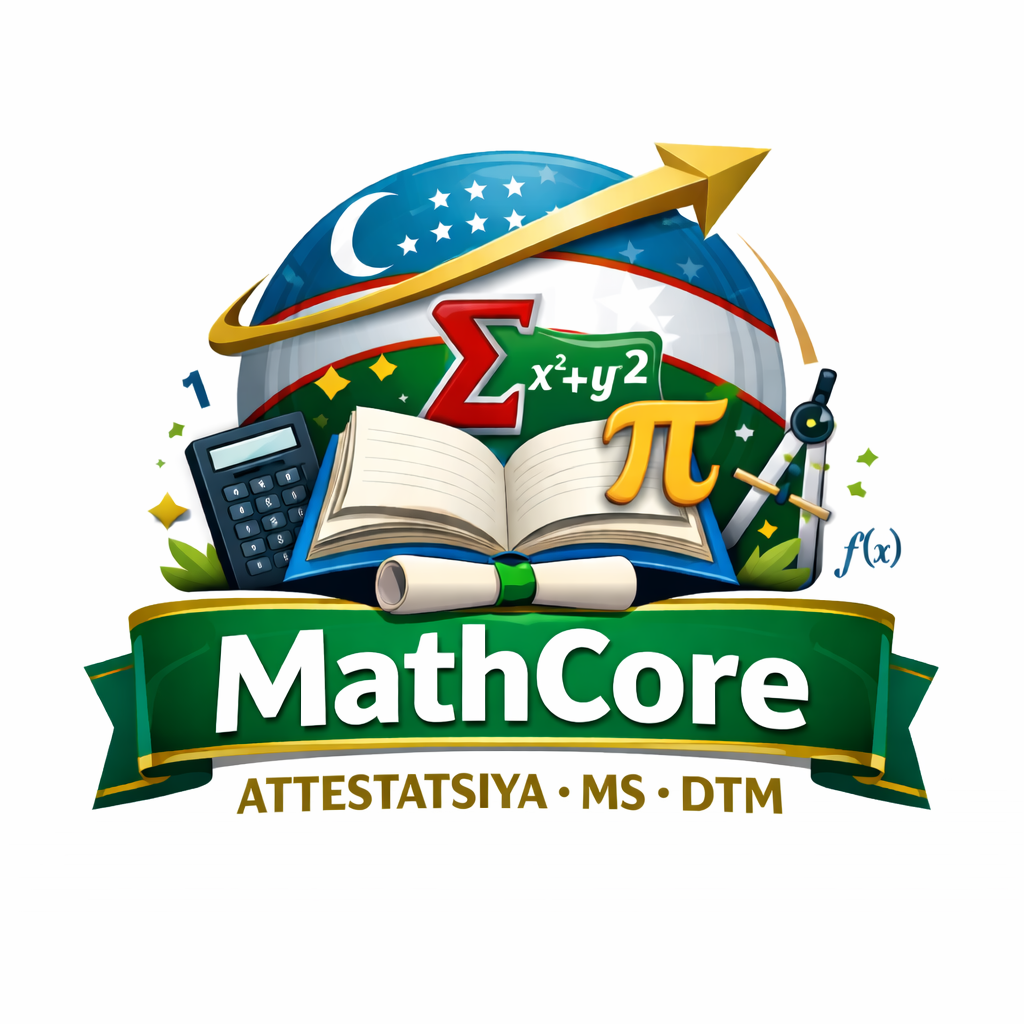
\includegraphics[width=0.2\textwidth]{logo.png} \\[5mm]
    \textcolor{gray}{\small Telegram: \href{https://t.me/Math_Core_Dtm_MS_Att}{@Math\_Core\_Dtm\_MS\_Att}}
\end{center}
\vspace{5mm}

% Задача 1
\begin{questionbox}{1}
    Определите, верны или неверны следующие утверждения:
    \begin{enumerate}
        \item[(I)] Если стороны треугольника равны \(a, b, c\), а полупериметр \(p\), то площадь \(S = \sqrt{p(p-a)(p-b)(p-c)}\).
        \item[(II)] Около четырёхугольника, у которого суммы противоположных сторон равны, можно описать окружность.
        \item[(III)] Около четырёхугольника, у которого суммы противоположных углов равны \(180^\circ\), можно описать окружность.
    \end{enumerate}
    \begin{options}
        \item I – неверно, II – неверно, III – верно
        \item I – неверно, II – неверно, III – неверно
        \item I – верно, II – неверно, III – верно
        \item I – верно, II – верно, III – неверно
    \end{options}
\end{questionbox}

% Задача 2
\begin{questionbox}{2}
    Вычислите: \(\sqrt{11 - 2\sqrt{30}} - \sqrt{11 + 2\sqrt{30}}\).
    \begin{options}
        \item \(-2\sqrt{5}\)
        \item \(-2\sqrt{6}\)
        \item \(2\sqrt{5}\)
        \item \(2\sqrt{6}\)
    \end{options}
\end{questionbox}

% Задача 3
\begin{questionbox}{3}
    Найдите сумму двузначных чисел, имеющих ровно три натуральных делителя.
    \begin{options}
        \item 49
        \item 74
        \item 78
        \item 199
    \end{options}
\end{questionbox}

% Задача 4
\begin{questionbox}{4}
    Если \((x - \frac{1}{3})(x + 2) = 0\), какие значения может принимать \((x - \frac{1}{3})\)?
    \begin{options}
        \item \(\frac{1}{3}\) и \(-2\)
        \item \(\frac{1}{3}\) и \(-7\)
        \item \(0\) и \(-7\)
        \item \(\frac{7}{3}\) и \(0\)
    \end{options}
\end{questionbox}

% Задача 5
\begin{questionbox}{5}
    Сколько действительных корней имеет уравнение \((x+1)^4 - 3(x^2+2x) - 13 = 0\)?
    \begin{options}
        \item 1
        \item 2
        \item 3
        \item 4
    \end{options}
\end{questionbox}

% Задача 6
\begin{questionbox}{6}
    На рисунке изображены графики функций \(y = f(x)\), \(y = g(x)\) и \(y = h(x)\). 
    Площади \(A_1 = 1\) см\(^2\), \(A_2 = 3\) см\(^2\), \(A_3 = 9\) см\(^2\). 
    Найдите значение \(\int_a^c (h(x)-g(x))\,dx + \int_b^d (f(x)-h(x))\,dx\).
\begin{dd}
        \centering
        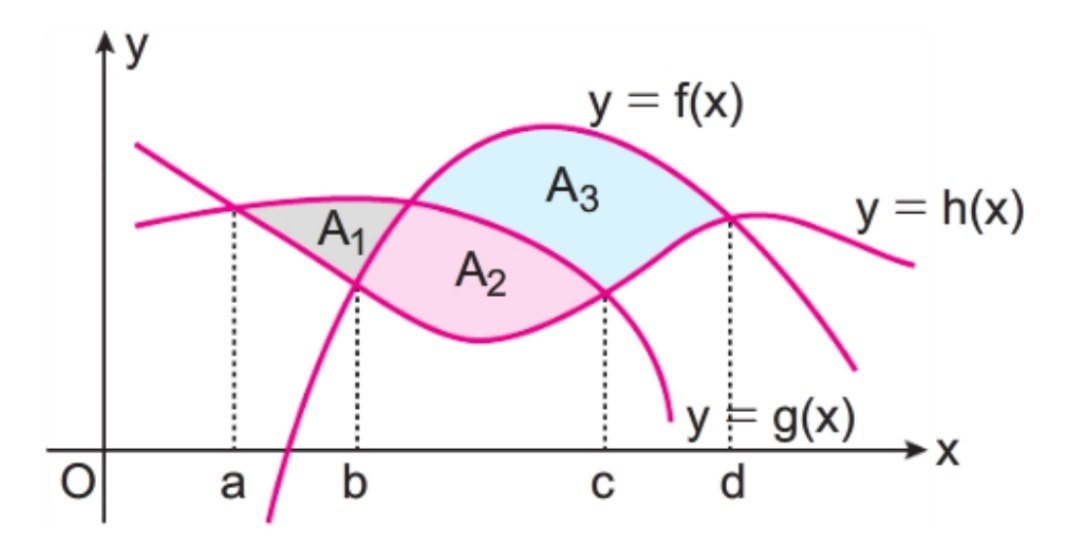
\includegraphics[width=0.5\linewidth]{qe.png}
    \end{dd}
        \begin{options}
        \item 5
        \item 12
        \item 8
        \item 13
    \end{options}
\end{questionbox}

% Задача 7
\begin{questionbox}{7}
    На день рождения ожидается 4 или 5 гостей. На какое наименьшее количество равных кусков можно разрезать круглый торт, чтобы его хватило в обоих случаях?
    \begin{options}
        \item 5
        \item 12
        \item 8
        \item 20
    \end{options}
\end{questionbox}

% Задача 8
\begin{questionbox}{8}
    Найдите \(\text{НОК}\left( \frac{4}{5}, \frac{5}{6},\frac{6}{7} \right)\)
    \begin{options}
        \item \(\frac{1}{210}\)
        \item \(\frac{4}{7}\)
        \item 120
        \item 60
    \end{options}
\end{questionbox}

% Задача 9
\begin{questionbox}{9}
    \(f(x) = (\sin x)^x\). Найдите \(f'\left(\frac{\pi}{2}\right)\).
    \begin{options}
        \item 0
        \item 2
        \item \(\ln 2\)
        \item нельзя определить
    \end{options}
\end{questionbox}

% Задача 10
\begin{questionbox}{10}
    На сторонах треугольника \(ABC\) отмечены 8 точек (см. рисунок). Какова вероятность того, что случайно выбранный треугольник с вершинами в этих точках имеет одну сторону, лежащую на стороне \(AB\)?
\begin{dd}
        \centering
        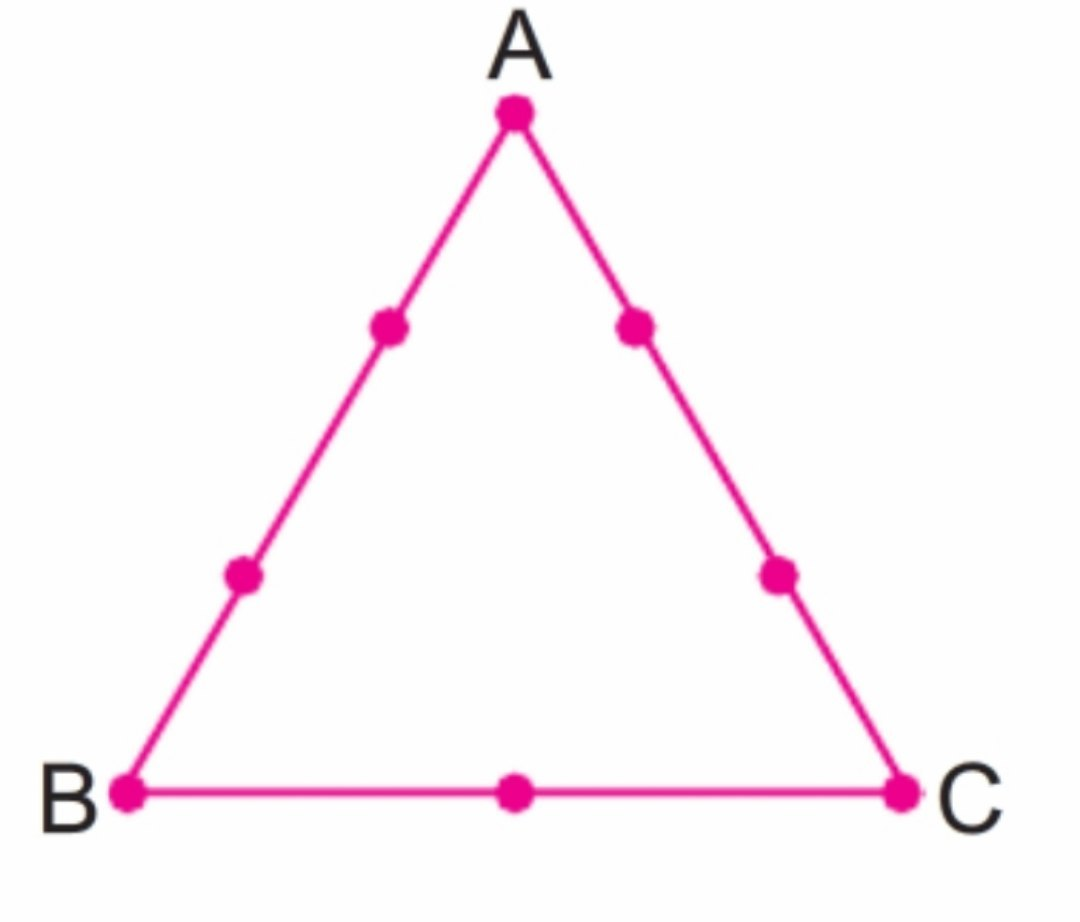
\includegraphics[width=0.3\linewidth]{ffs.png}
    \end{dd}
        \begin{options}
        \item \(\frac{16}{47}\)
        \item \(\frac{18}{47}\)
        \item \(\frac{20}{47}\)
        \item \(\frac{24}{47}\)
    \end{options}
\end{questionbox}

% Задача 11
\begin{questionbox}{11}
    Решите уравнение: \(\left( (\sqrt[3]{x})^{-1/2} \right)^{\frac{6}{5}} = \left( (1/\sqrt{x})^{-4/3} \right)^{\frac{6}{5}}\).
    \begin{options}
        \item \(\sqrt[3]{2}\)
        \item 1
        \item \(\sqrt[3]{6}\)
        \item \(\sqrt[3]{4}\)
    \end{options}
\end{questionbox}

% Задача 12
\begin{questionbox}{12}
    Найдите решение неравенства \(\cos^2 x - \frac{\sqrt{2}}{2} \le \sin^2 x\) на отрезке \([0; \pi]\).
    \begin{options}
        \item \(\left[\frac{\pi}{6}, \frac{5\pi}{6}\right]\)
        \item \(\left[\frac{\pi}{8}, \frac{7\pi}{8}\right]\)
        \item \(\left[\frac{\pi}{4}, \frac{3\pi}{8}\right]\)
        \item \(\left[\frac{\pi}{12}, \frac{5\pi}{12}\right]\)
    \end{options}
\end{questionbox}

% Задача 13
\begin{questionbox}{13}
    Предприниматель продал кусок ткани 9 покупателям: первому — \(\frac{1}{9}\) всего куска, второму — \(\frac{1}{8}\) остатка, третьему — \(\frac{1}{7}\) нового остатка, и так далее. Восьмому — половину остатка, а девятому — оставшиеся 40 метров. Сколько метров было в куске?
    \begin{options}
        \item 240
        \item 320
        \item 360
        \item 440
    \end{options}
\end{questionbox}

% Задача 14
\begin{questionbox}{14}
    \(x = 2^{22} \cdot 5^{17} \cdot 10^{3} \cdot 5^{5}\). Сколько цифр в числе \(x\)?
    \begin{options}
        \item 25
        \item 26
        \item 27
        \item 28
    \end{options}
\end{questionbox}

% Задача 15
\begin{questionbox}{15}
    Решите уравнение: \(2^{x+1} + 2^{x-1} - 3^{x-1} = 3^{x-2} - 2^{x-3} + 2 \cdot 3^{x-3}\).
    \begin{options}
        \item \(x = 2\)
        \item \(x = 3\)
        \item \(x = 4\)
        \item \(x = 5\)
    \end{options}
\end{questionbox}

% Задача 16
\begin{questionbox}{16}
    Найдите остаток от деления \(3^{80} + 7^{80}\) на 11.
    \begin{options}
        \item 0
        \item 2
        \item 7
        \item 10
    \end{options}
\end{questionbox}

% Задача 17
\begin{questionbox}{17}
    На рисунке изображена единичная окружность. Решение какого неравенства показано?
\begin{dd}
        \centering
        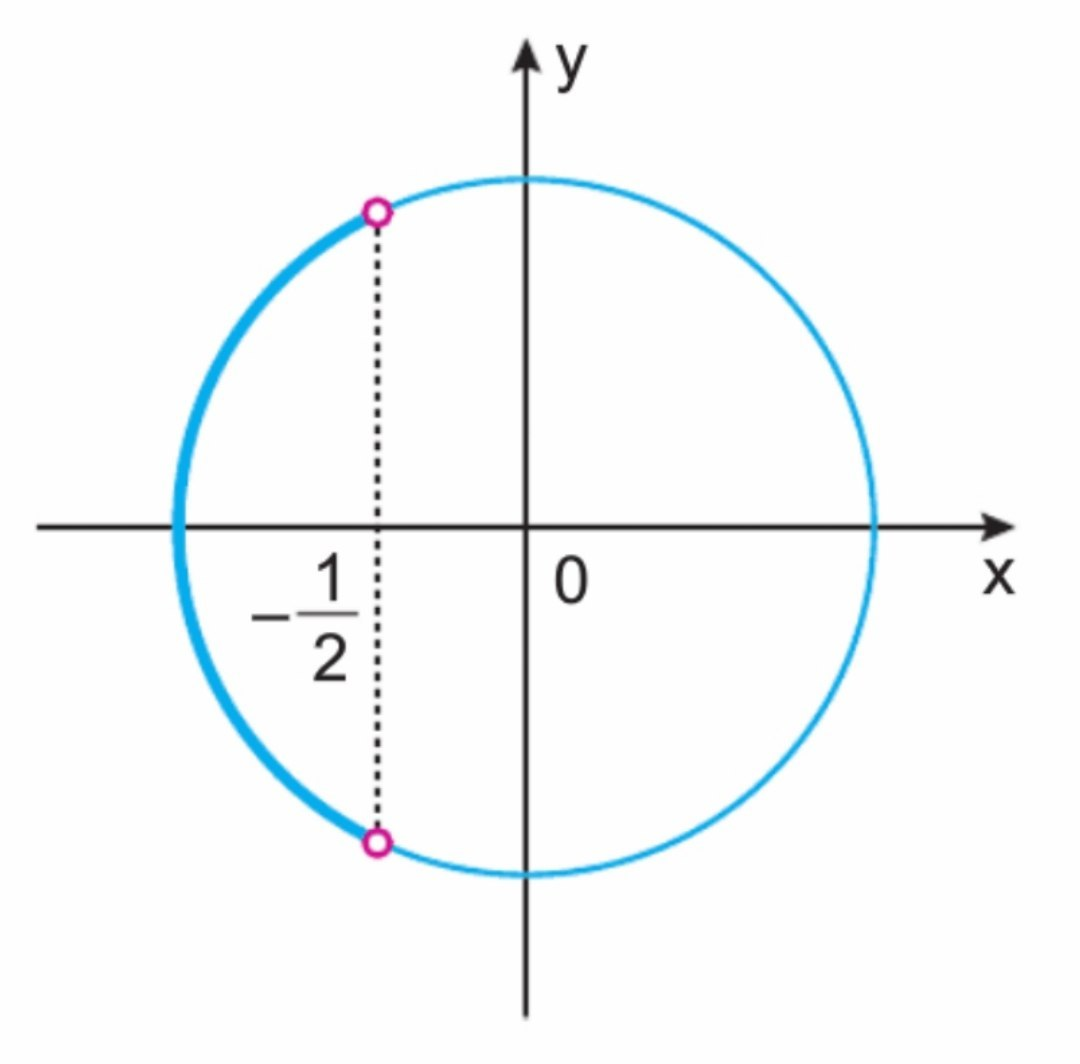
\includegraphics[width=0.3\linewidth]{fjakfa.png}
    \end{dd}
        \begin{options}
        \item \(\cos x < -\frac{1}{2}\)
        \item \(\sin x > -\frac{1}{2}\)
        \item \(\cos x > -\frac{1}{2}\)
        \item \(\sin x < -\frac{1}{2}\)
    \end{options}
\end{questionbox}

% Задача 18
\begin{questionbox}{18}
    Упростите: \(\frac{\lg(7 - 4\sqrt{3})}{\lg(2 - \sqrt{3})}\) 
    \begin{options}
        \item 2
        \item 1
        \item \(\sqrt{3}\)
        \item \(-1\)
    \end{options}
\end{questionbox}

% Задача 19
\begin{questionbox}{19}
    \(f(x) = \begin{cases} x^2 - 2x + 4, & x > 1 \\ x^3 + 2x, & x \le 1 \end{cases}\).
    Найдите \(\lim_{x \to 0} f(x) + \lim_{x \to 2} f(x) + \lim_{x \to 1} f(x)\).
    \begin{options}
        \item 9
        \item 7
        \item 6
        \item 4
    \end{options}
\end{questionbox}

% Задача 20
\begin{questionbox}{20}
    Сколько целых решений имеет неравенство
    \[
    \sqrt[3]{x^2 - 10x + 16} \cdot (x+3)^2 \cdot \log_{2x-x^2}(2^{x^2}) \le 0?
    \]
    \begin{options}
        \item 0
        \item 6
        \item 7
        \item 1
    \end{options}
\end{questionbox}

% Задача 21
\begin{questionbox}{21}
    В арифметической прогрессии \(S_{n+2} - S_{n-2} = 33\) и \(S_n - S_{n-4} = 9\). Найдите разность прогрессии.
    \begin{options}
        \item 1
        \item 2
        \item 3
        \item 4
    \end{options}
\end{questionbox}

% Задача 22
\begin{questionbox}{22}
    На диаграмме показана зависимость пройденного автомобилем пути (км) от времени (час). Найдите медиану расстояний, пройденных за каждый час (в конце каждого часа).
\begin{dd}
        \centering
        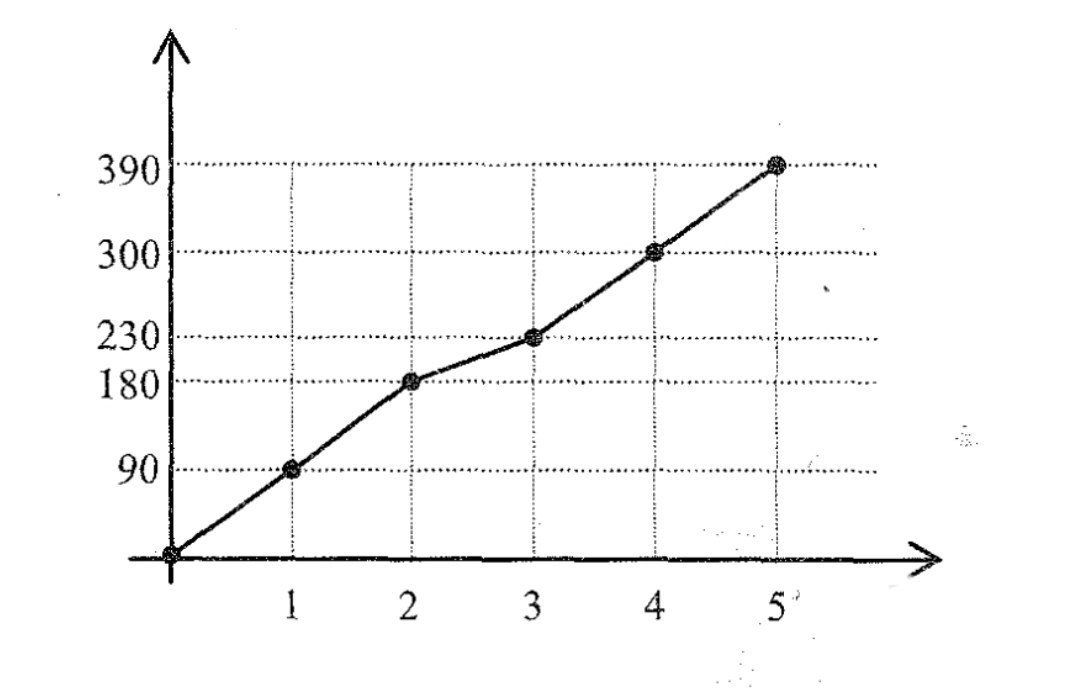
\includegraphics[width=0.4\linewidth]{dad.png}
    \end{dd}
        \begin{options}
        \item 230
        \item 90
        \item 180
        \item 390
    \end{options}
\end{questionbox}

% Задача 23
\begin{questionbox}{23}
    В школьной столовой есть 4 вида пирожных. Сколькими способами ученик может выбрать 5 пирожных?
    \begin{options}
        \item 5
        \item 20
        \item 56
        \item 60
    \end{options}
\end{questionbox}

% Задача 24
\begin{questionbox}{24}
    Остаток от деления многочлена \(P(x-2)\) на \((x-4)\) равен 2022. Найдите остаток от деления \(P(x+3)\) на \((x+1)\).
    \begin{options}
        \item 2022
        \item 1011
        \item 0
        \item нельзя определить
    \end{options}
\end{questionbox}

% Задача 25
\begin{questionbox}{25}
    Вычислите сумму: \(\frac{2}{3} + \frac{5}{6} + \frac{11}{12} + \frac{23}{24} + \dots + \frac{767}{768}\) 
    \begin{options}
        \item \(\frac{6401}{768}\)
        \item \(\frac{939}{128}\)
        \item \(\frac{1963}{256}\)
        \item \(\frac{1963}{768}\)
    \end{options}
\end{questionbox}

% Задача 26
\begin{questionbox}{26}
    Найдите значение выражения: \(\sin 20^\circ \cdot \sin 40^\circ \cdot \sin 80^\circ\).
    \begin{options}
        \item \(\frac{1}{8}\)
        \item \(\frac{1}{4}\)
        \item \(\frac{\sqrt{3}}{8}\)
        \item \(\frac{1}{16}\)
    \end{options}
\end{questionbox}

% Задача 27
\begin{questionbox}{27}
   Если \(f(x) = e^{(\ln x^4)}\) ), найдите \(f''(1)\).
    \begin{options}
        \item 9
        \item 10
        \item 12
        \item 13
    \end{options}
\end{questionbox}

% Задача 28 (первая)
\begin{questionbox}{28}
    Найдите сумму всех членов последовательности \(a_n = \frac{2}{3^{n}}\)
    
    \begin{options}
        \item нельзя определить
        \item \(\frac{1}{3}\)
        \item \(\frac{2}{3}\)
        \item 1
    \end{options}
\end{questionbox}

% Задача 29
\begin{questionbox}{29}
    В полуокружность радиуса 6 см вписан прямоугольный треугольник \(CHB\) (см. рисунок). Найдите наибольшую возможную площадь треугольника \(CHB\).
\begin{dd}
        \centering
        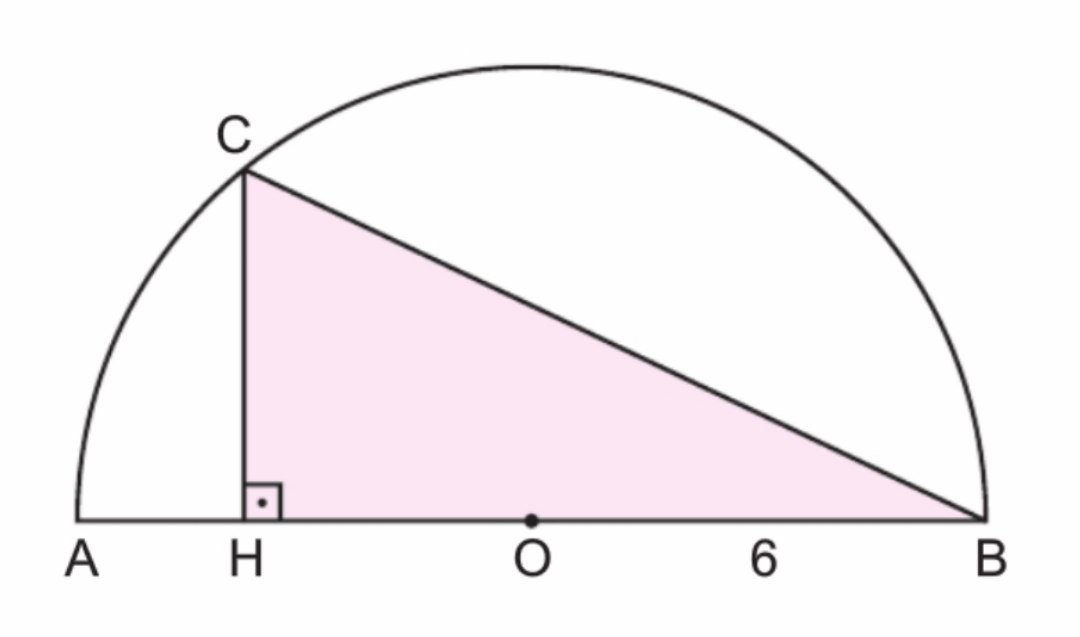
\includegraphics[width=0.3\linewidth]{dsw.png}
    \end{dd}
        \begin{options}
        \item \(\frac{24\sqrt{2}}{5}\)
        \item \(\frac{27\sqrt{3}}{2}\)
        \item \(\frac{32\sqrt{2}}{5}\)
        \item \(\frac{35\sqrt{2}}{2}\)
    \end{options}
\end{questionbox}

% Задача 30
\begin{questionbox}{30}
    Внутренние углы треугольника равны \(a, b, c\). Известно, что треугольник не прямоугольный. Какое из следующих утверждений неверно?
    \begin{options}
        \item \(\cos a = \sin\frac{b+c}{2}\)
        \item \(\sin a = \sin(b+c)\)
        \item \(\tg b = -\tg(a+c)\)
        \item \(\ctg(b+c) = \ctg a\)
    \end{options}
\end{questionbox}

% Задача 31
\begin{questionbox}{31}
    Точка \(P(2; -3)\) лежит вне окружности \((x+4)^2 + (y-5)^2 = r^2\). Найдите наибольшее целое значение \(r\).
    \begin{options}
        \item 7
        \item 8
        \item 9
        \item 10
    \end{options}
\end{questionbox}

% Задача 32
\begin{questionbox}{32}
    В треугольнике \(ABC\) на медиане \(AD\) выбрана точка \(K\) такая, что \(AK = BC\) и \(\angle ADC = 120^\circ\). Найдите \(\frac{AB}{KC}\) (в оригинале: найти AB, но скорее отношение).
    \begin{options}
        \item 1
        \item \(\sqrt{3}\)
        \item \(\frac{1}{\sqrt{3}}\)
        \item \(\sqrt{2}\)
    \end{options}
\end{questionbox}

% Задача 33
\begin{questionbox}{33}
    В прямоугольном треугольнике \(ABC\) (см. рисунок) \(BD = 4\), \(AC = 18\), \(AD\) — биссектриса. Найдите площадь треугольника \(ADC\).
\begin{dd}
        \centering
        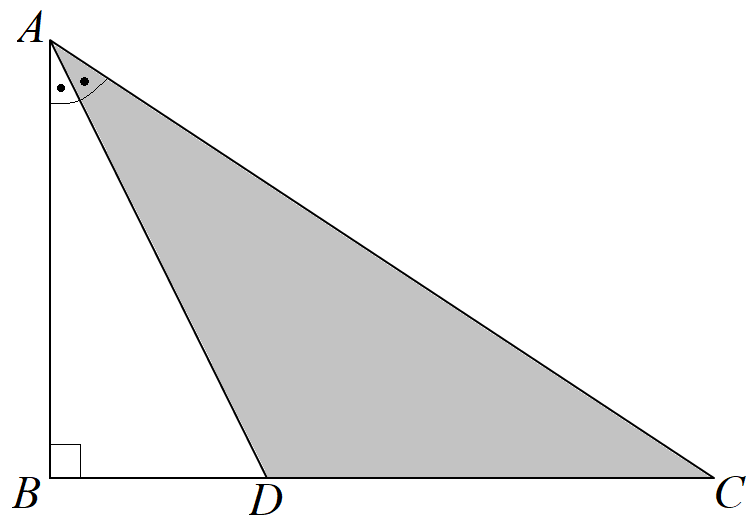
\includegraphics[width=0.3\linewidth]{jfa.png}
    \end{dd}
        \begin{options}
        \item 24
        \item 36
        \item 48
        \item 60
    \end{options}
\end{questionbox}

% Задача 34
\begin{questionbox}{34}
    В цилиндр вписана правильная треугольная призма, а в эту призму вписан цилиндр. Найдите отношение объёма большого цилиндра к объёму малого.
    \begin{options}
        \item 4
        \item 3
        \item 6
        \item 2
    \end{options}
\end{questionbox}

% Задача 35
\begin{questionbox}{35}
    В полусферу радиуса 9 см вписан цилиндр (см. рисунок). Какой должна быть высота цилиндра, чтобы его объём был наибольшим?
\begin{dd}
        \centering
        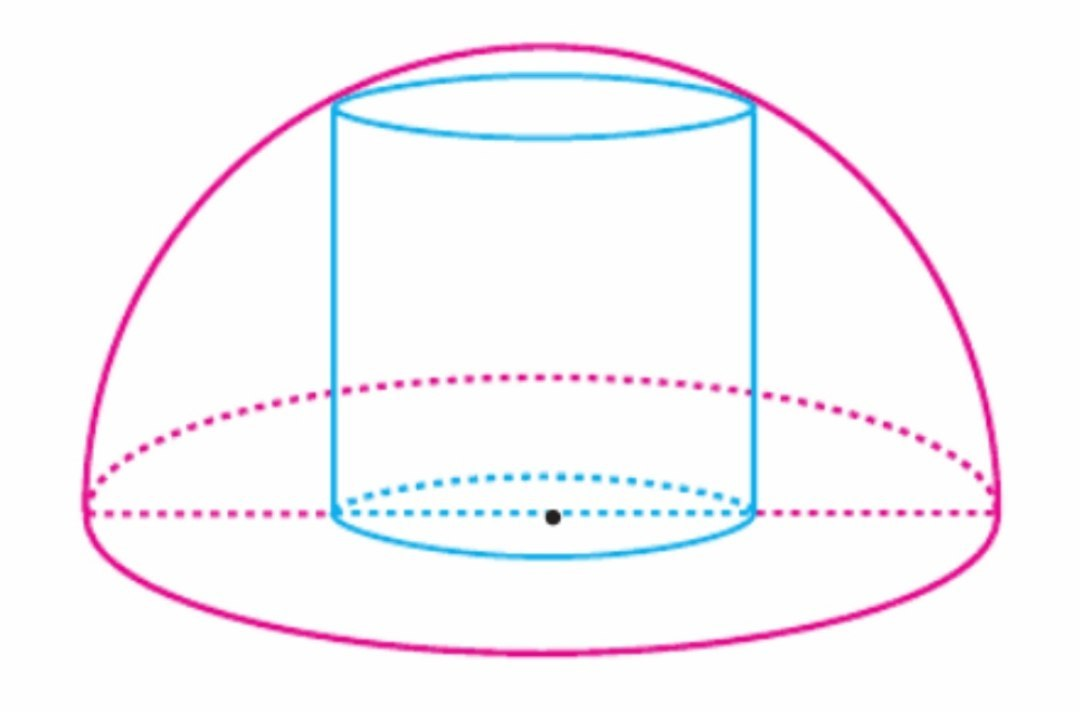
\includegraphics[width=0.3\linewidth]{has.png}
    \end{dd}
        \begin{options}
        \item \(2\sqrt{3}\)
        \item \(3\sqrt{3}\)
        \item 3
        \item 4
    \end{options}
\end{questionbox}

\end{document}